\section[Notebook 1970-15: the Möbius function of the lattice of subspaces]{Notebook 1970-15: the Möbius function of the lattice of subspaces\protect\verifie{Notebook1970_15}}\label{sec:quillen-1970-15}

\emph{Context.} In September 1970, \carnet{1970}{15} compares the cohomology of a group in a topos with that of its points. On pages~21--22, Quillen inverts Euler characteristics over the isotropy types of an action, with Möbius coefficients, and checks the formula for an elementary abelian group acting on a point. In rank~$3$, the check reduces to the identity $1 - (q^2 + q + 1) + q(q^2 + q + 1) - q^3 = 0$: the alternating sum, over the subspaces $W$ of a space of dimension $n$ over $\mathbf F_q$, of $(-1)^{\dim W} q^{\binom{\dim W}{2}}$ is zero for $n \ge 1$, since $(-1)^k q^{\binom{k}{2}}$ is the value of the Möbius function of the lattice of subspaces on an interval of rank~$k$. Figure~\ref{fig:quillen-1970-15} shows the case $n = 3$, $q = 2$.

\emph{Intuition.} The number of subspaces of dimension $k$ is the Gaussian binomial coefficient $\left[\begin{smallmatrix} n \\ k \end{smallmatrix}\right]_q$, and these coefficients satisfy Gauss's binomial theorem $\prod_{i < n}(1 + q^i t) = \sum_k q^{\binom{k}{2}} \left[\begin{smallmatrix} n \\ k \end{smallmatrix}\right]_q t^k$. For $t = -1$, the factor $i = 0$ of the product vanishes.


\begin{figure}[htbp]
\centering
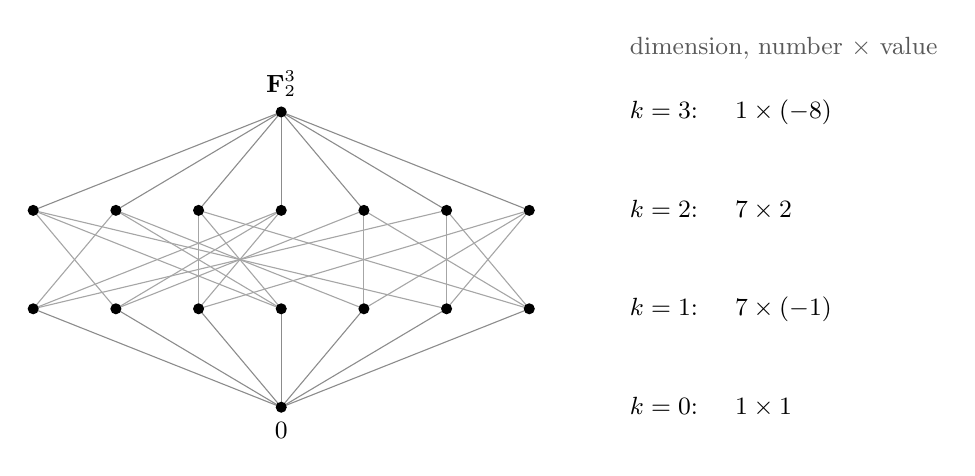
\begin{tikzpicture}[x=1.05cm, y=1.25cm, every node/.style={font=\small}]
\foreach \i in {0,...,6} {
  \coordinate (d\i) at ({\i-3},1);
  \coordinate (p\i) at ({\i-3},2);
  \draw[black!45] (0,0) -- (d\i);
  \draw[black!45] (p\i) -- (0,3);
}
\foreach \i/\j in {0/1,0/3,0/5,1/0,1/3,1/4,2/2,2/3,2/6,3/0,3/1,3/2,4/1,4/4,4/6,5/0,5/5,5/6,6/2,6/4,6/5} { \draw[black!35] (d\i) -- (p\j); }
\fill (0,0) circle (2pt); \fill (0,3) circle (2pt);
\foreach \i in {0,...,6} { \fill (d\i) circle (2pt); \fill (p\i) circle (2pt); }
\node[below=2pt] at (0,0) {$0$};
\node[above=2pt] at (0,3) {$\mathbf F_2^3$};
\foreach \y/\t in {0/{1 \times 1}, 1/{7 \times (-1)}, 2/{7 \times 2}, 3/{1 \times (-8)}} {
  \node[anchor=west] at (4.1,\y) {$k = \y$: \quad $\t$};
}
\node[anchor=west, black!65] at (4.1,3.65) {dimension, number $\times$ value};
\end{tikzpicture}
\caption{The lattice of subspaces of $\mathbf F_2^3$: the zero subspace, seven lines, seven planes and the whole space; each plane contains three lines. On the right, for each dimension $k$, the number $\left[\begin{smallmatrix} 3 \\ k \end{smallmatrix}\right]_2$ of subspaces and the value $(-1)^k q^{\binom{k}{2}}$ of the Möbius function between $0$ and a subspace of dimension $k$, for $q = 2$. The sum $1 - 7 + 14 - 8$ is zero: this is the identity of page~22 for $q = 2$.}
\label{fig:quillen-1970-15}
\end{figure}

\begin{encadre}
\begin{theoreme}[Quillen, notebook 1970-15, pp.~21--22]\label{thm:quillen-1970-15}
Let $R$ be a commutative ring and $q \in R$. Define $\left[\begin{smallmatrix} n \\ k \end{smallmatrix}\right]_q$ by $\left[\begin{smallmatrix} n \\ 0 \end{smallmatrix}\right] = 1$, $\left[\begin{smallmatrix} 0 \\ k + 1 \end{smallmatrix}\right] = 0$ and $\left[\begin{smallmatrix} n + 1 \\ k + 1 \end{smallmatrix}\right] = \left[\begin{smallmatrix} n \\ k \end{smallmatrix}\right] + q^{k+1} \left[\begin{smallmatrix} n \\ k + 1 \end{smallmatrix}\right]$. Then, for all $t \in R$,
\[
\prod_{i = 0}^{n - 1} (1 + q^i t) = \sum_{k = 0}^{n} q^{\binom{k}{2}} \begin{bmatrix} n \\ k \end{bmatrix}_q t^k,
\qquad\text{and}\qquad
\sum_{k = 0}^{n} (-1)^k q^{\binom{k}{2}} \begin{bmatrix} n \\ k \end{bmatrix}_q = 0 \quad (n \ge 1).
\]
For $n = 3$, this is the identity of page~22.
\end{theoreme}
\end{encadre}

\begin{proof}
By induction on $n$, for all $t$ at once. Write $\prod_{i \le n}(1 + q^i t) = (1 + t) \prod_{i < n}(1 + q^i (qt))$ and apply the induction hypothesis to $qt$. The coefficient of $t^{k+1}$ in the product with $1 + t$ is $q^{\binom{k}{2} + k}\left[\begin{smallmatrix} n \\ k \end{smallmatrix}\right] + q^{\binom{k+1}{2} + k + 1}\left[\begin{smallmatrix} n \\ k + 1 \end{smallmatrix}\right]$, that is $q^{\binom{k+1}{2}}\left[\begin{smallmatrix} n + 1 \\ k + 1 \end{smallmatrix}\right]$ by Pascal's recurrence, since $\binom{k+1}{2} = \binom{k}{2} + k$ and $\left[\begin{smallmatrix} n \\ n + 1 \end{smallmatrix}\right] = 0$. For $t = -1$ and $n \ge 1$, the factor $1 + q^0 \cdot (-1)$ vanishes.
\end{proof}

\begin{sloppypar}
\noindent\emph{Verification in Lean.} The coefficients are \texttt{qBinom}, with \texttt{qBinom\_eq\_zero\_of\_lt}; the binomial theorem is \texttt{prod\_one\_add\_eq\_sum}, the alternating sum is \texttt{sum\_alternating\_eq\_zero}, and the check of the page is \texttt{quillen\_check\_rank\_three}, in \href{\leanblobmain/Notebook1970_15.lean}{\texttt{Notebook1970\_15.\allowbreak{}lean}}. mathlib has no Gaussian binomial coefficients; the file defines them.
\end{sloppypar}

Not formalized: the counting of subspaces of $\mathbf F_q^n$ by the $\left[\begin{smallmatrix} n \\ k \end{smallmatrix}\right]_q$, and Möbius inversion over isotropy types. The proposition of page~14 (a pro-$\ell$-group has cohomology of finite type if and only if it has an open subgroup of finite cohomology) would require the cohomology of profinite groups, absent from mathlib; it is not attempted.

\litterature{found in the literature: P.~Hall (1936); Rota, \q{On the foundations of combinatorial theory I} (1964); Stanley, \emph{Enumerative Combinatorics}~I, 3.10. The statement is classical; the edition does not present it as new.}
